\documentclass{article}
\usepackage{siunitx} 
\usepackage{graphicx}
\usepackage{natbib}
\usepackage{amsmath} 

\setlength\parindent{0pt}

\renewcommand{\labelenumi}{\alph{enumi}.}

%\usepackage{times} 

%----------------------------------------------------------------------------------------
%	DOCUMENT INFORMATION
%----------------------------------------------------------------------------------------

\title{Práctica 10 \\ Programación Concurrente y de Tiempo Real \\Universidad de Cádiz} % Title

\author{Alejandro Serrano Fernández} % Author name

\date{\today} % Date for the report

\begin{document}

\maketitle % Insert the title, author and date


%----------------------------------------------------------------------------------------
%	SECTION 1
%----------------------------------------------------------------------------------------
\section{Ejercicio 1}
Para calcular el tiempo que tarda mi computadora en calcular el número de primos que hay en un rango dado, cabe destacar que los siguientes datos han sido obtenidos a través de un portátil equipado con un i7-7700hq de 4 núcleos y 8 threads. 

Bien, como podemos observar, para un número bajo de hilos, obtiene mejores resultados la versión realizada con Runnable, aunque a partir de 6 hilos, cabe destacar que ambos comienzan a obtener resultados similares en lo que a tiempo se refiere. Por tanto, si estamos en la duda de elegir una opción u otra, pues dependerá del número de hilos que vayamos a utilizar. Si utilizamos pocos hilos nos conviene con Runnable. Si utilizamos más hilos, podremos usar cualquiera de las dos versiones. 


\begin{center}
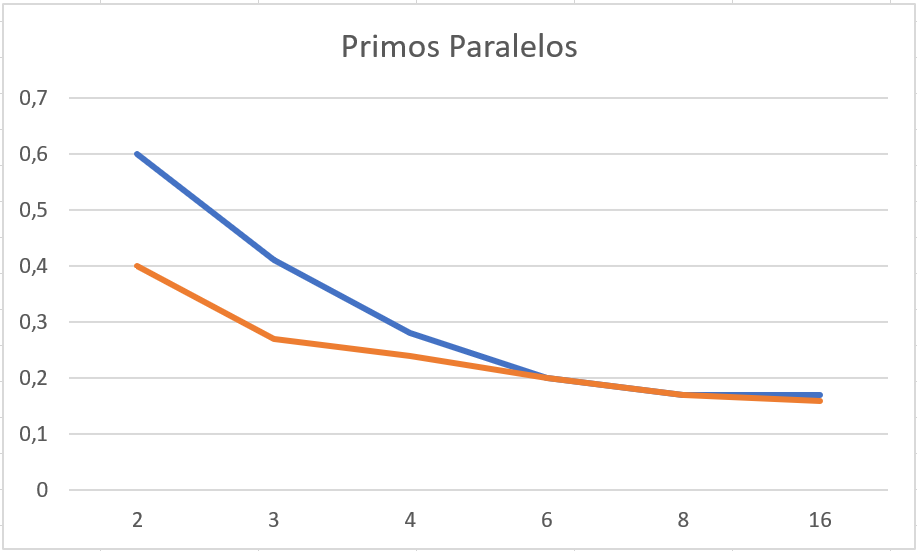
\includegraphics[scale=0.5]{grafica.png}
\end{center}
En azul nos encontramos con la implementación en MPJ y en naranja con la implementación en Runnable. He usado un rango de búsqueda de 1000000 números. En total obtenemos que hay 78498 números primos
\end{document}



